\documentclass[openany]{book}
\usepackage[utf8]{inputenc}
\usepackage{verbatim}
%%%%%%%%%%%%%%%%%%%%%%%

%%%%%%%%%%%%%%%%%%%%%%%
% HOLA PACO
% ESTE ES EL ARCHIVO DE LAS DEFINICIONES ESTRUCTURALES
% VERSION 1.1 NOMÁS
%
% AUTOR ORIGINAL:
% EDUARDO (CHITO) BELMONTE GUILLAMÓN
%
% ESTE ARCHIVO ES COMUNISTA, PUEDES COMPARTIRLO SI QUIERES
%%%%%%%%%%%%%%%%%%%%%%%

%----------------------------------
%     PAQUETICOS QUE SE USAN
%----------------------------------

%--------------------------
%    PARA USAR INKSCAPE
%---------------------------
\usepackage{import}
\usepackage{hyperref}
\usepackage{xifthen}
\usepackage{pdfpages}
\usepackage{transparent}

\newcommand{\incfig}[1]{%
    \def\svgwidth{\columnwidth}
    \import{./figures/}{#1.pdf_tex}
}

\newcommand{\custincfig}[2]{%
    \def\svgwidth{#1}
    \import{./figures/}{#2.pdf_tex}
}
\newcommand{\textnexttofig}[3]{
  \begin{minipage}[l]{0.45\textwidth}
    \custincfig{#1}{#2}
  \end{minipage}
  \begin{minipage}[l]{0.45\textwidth}
    #3
  \end{minipage}
}

%%%%%%%%% FIN DEL INKSCAPE

\usepackage{parskip} % Pa parrafos wapos
\setlength{\parindent}{0.5cm} % Pa la sangría
\usepackage{graphicx} % Pa meter las imágenes
\graphicspath{{Images/}} % La ruta a las imágenes

\usepackage{tikz} % Pa dibujar cosichuelas guapas

\usepackage[spanish]{babel} % PA QUE ESTÉ EN ESPAÑOL NOMÁS

\usepackage{enumitem} % Para personalizar las LISTAS YEAH

\setlist{nolistsep} % Pa que las listas estén junticas

\usepackage{booktabs} % Esta sirve para hacer tablas fancy con multicolumns y tal pero no tengo ni puta idea de usarla

\usepackage{xcolor} % PA DEFINIR LOS COLORINES
\definecolor{turquoise}{RGB}{21,103,112} % Es un turquesica así formal
\definecolor{violet}{RGB}{ 110, 6, 187 } % Color maricón

%-------------------------------------------------
%     MÁRGENES
%-------------------------------------------------

\usepackage{geometry}
\geometry{
    top=3cm,
    bottom=3cm,
    left=3cm,
    right=3cm,
    headheight=14pt,
	footskip=1.4cm,
	headsep=10pt,
}

\usepackage{avant} % Esto es una fuente para encabezados

%\usepackage{mathptmx} % Usar simbolitos matemáticos chulos

\usepackage{microtype} % Para fuentes de maricones

\usepackage[utf8]{inputenc} % Pa los acentos

\usepackage[T1]{fontenc}

%-------------------------------------------------
% Bibliografía e índice
%-------------------------------------------------

\usepackage{makeidx} % Pa hacer un índice
\makeindex

\usepackage{titletoc}   % Para manipular la tabla de contenidos

\contentsmargin{0cm}    % Para eliminar el margen por defecto

\usepackage{titlesec} % Pa cambiar los titulos skere

\titleformat
{\chapter} % command
[display] % shape
{\centering\bfseries\Huge\normalfont} % format
{\color{turquoise}  {\normalsize\MakeUppercase{Capítulo} \thechapter }} % label
{-0.5cm} % sep
{
    \color{turquoise}
    \rule{\textwidth}{3pt}
    \vspace{1ex}
    \centering
    \setcounter{ex}{0}
    \setcounter{dummy}{0}
} % before-code
[
\vspace{-0.5cm}%
\rule{\textwidth}{3pt}
] % after-code


\titleformat{\part}
[display]
{\centering\bfseries\Huge\normalfont}
{\color{turquoise} {\normalsize \MakeUppercase{Asignatura}}}
{0pt}
{\color{turquoise}
\vspace{-0.6cm}
\rule{\textwidth}{3pt}
\vspace{1ex}
\setcounter{chapter}{0}
\setcounter{section}{0}
\setcounter{dummy}{0}
\centering
}


\titleformat{\section}
{\normalfont\Large\bfseries}{\color{turquoise}\thesection\ - }{0.5em}{}

\usepackage{fancyhdr}   % Necesario para el encabezado y el pie de página

\pagestyle{fancy}   %Para modificar los encabezados
\fancyhf{}          %Para eliminar los encabezados y pies de página por defecto.
\fancyhead[LE,RO]{\sffamily\normalsize\thepage}
\fancyfoot[C]{Ampliación de Probabilidad}
%HACER

\usepackage{amsmath,amsfonts,amssymb,amsthm,cancel} % PARA LAS MATES

%   LINEA 199, HACER CAPULLADAS

\newtheoremstyle{turquoisebox}
{0pt} %Espacio encima
{0pt} %Espacio abajo
{\normalfont} % Fuente del cuerpo
{} % Cantidad de identado
{\small\ssfamily\color{turquoise}} % Fuente en la que pone "TEOREMA"
{:} % Puntuación tras el teorema
{0.25em} %Espacio tras el teorema
{\thmname{#1}\thmnumber{#2}} %No sé si esto funciona


\newcounter{dummy}
\newcounter{ex}
\newtheorem{teoremote}[dummy]{\color{turquoise}Teorema}
\newtheorem{propositiont}{\color{turquoise}Proposición}[section]
\newtheorem{lemmat}{\color{turquoise}Lema}[section]
\newtheorem{definitionT}{\color{turquoise}Definición}[section]
\newtheorem{exerciseT}[ex]{Ejercicio}
\newtheorem{examplote}[ex]{\color{turquoise}Ejemplo}
\newtheorem{methodT}[dummy]{\color{turquoise}Método}


\RequirePackage[framemethod=default]{mdframed} % Required for creating the theorem, definition, exercise and corollary boxes

%Caja de teoremas

\newmdenv[skipabove=7pt,
skipbelow=7pt,
backgroundcolor=black!5,
linecolor=turquoise,
innerleftmargin=5pt,
innerrightmargin=5pt,
innertopmargin=5pt,
leftmargin=0cm,
rightmargin=0cm,
linewidth=3pt,
innerbottommargin=5pt]{tBox}

\newmdenv[skipabove=7pt,
skipbelow=7pt,
backgroundcolor=black!5,
linecolor=turquoise,
innerleftmargin=5pt,
innerrightmargin=5pt,
innertopmargin=5pt,
leftmargin=0cm,
rightmargin=0cm,
linewidth=1pt,
innerbottommargin=5pt]{pBox}

\newmdenv[skipabove=7pt,
skipbelow=7pt,
backgroundcolor=violet!7,
linecolor=turquoise,
innerleftmargin=5pt,
innerrightmargin=5pt,
innertopmargin=5pt,
leftmargin=0cm,
rightmargin=0cm,
rightline=false,
topline=false,
bottomline=false,
linewidth=4pt,
innerbottommargin=5pt]{mBox}

\newmdenv[skipabove=7pt,
skipbelow=7pt,
rightline=false,
leftline=true,
topline=false,
bottomline=false,
linecolor=turquoise,
innerleftmargin=5pt,
innerrightmargin=5pt,
innertopmargin=0pt,
leftmargin=0cm,
rightmargin=0cm,
linewidth=4pt,
innerbottommargin=0pt]{dBox}

\newmdenv[skipabove=7pt,
skipbelow=7pt,
rightline=false,
leftline=true,
topline=false,
bottomline=false,
backgroundcolor=black!3,
linecolor=turquoise!50,
innerleftmargin=5pt,
innerrightmargin=5pt,
innertopmargin=0pt,
innerbottommargin=5pt,
leftmargin=0cm,
rightmargin=0cm,
linewidth=4pt]{eBox}

\newmdenv[skipabove=7pt,
skipbelow=7pt,
leftline=true,
topline=false,
rightline=false,
bottomline=false,
backgroundcolor=cyan!5,
linecolor=turquoise,
innerleftmargin=5pt,
innerrightmargin=5pt,
innertopmargin=0pt,
innerbottommargin=5pt,
leftmargin=0cm,
rightmargin=0cm,
linewidth=4pt]{exBox}

\newenvironment{theorem}{\begin{tBox}\begin{teoremote}}{\end{teoremote}\end{tBox}}
\newenvironment{proposition}{\begin{pBox}\begin{propositiont}}{\end{propositiont}\end{pBox}}
\newenvironment{lemma}{\begin{pBox}\begin{lemmat}}{\end{lemmat}\end{pBox}}
\newenvironment{method}{\begin{mBox}\begin{methodT}}{\end{methodT}\end{mBox}}
\newenvironment{definition}{\begin{dBox}\begin{definitionT}}{\end{definitionT}\end{dBox}}
\newenvironment{exercise}{\begin{eBox}\begin{exerciseT}}{\hfill{\color{black}}\end{exerciseT}\end{eBox}}
\newenvironment{example}{\begin{exBox}\begin{examplote}}{\end{examplote}\end{exBox}}
\newenvironment{demonstration}{\begin{flushright}
      \color{turquoise} \textbf{Demostración}
\end{flushright}
}{\begin{flushright}
  $\square$
\end{flushright}}

\usepackage{geometry}
\geometry{
    top=3cm,
    bottom=3cm,
    left=3cm,
    right=3cm,
    headheight=14pt,
	footskip=1.4cm,
	headsep=10pt,
}
\usepackage{graphicx}
\title{Ecuaciones en Derivadas Parciales y Series de Fourier}
\author{Colaboración estelar entre Paco Mora 
\includegraphics[scale=0.02]{cosmo} y Chito Belmonte 
\includegraphics[scale=0.13]{wanda}}
\date{\today}

\begin{document}
\maketitle

\tableofcontents

\textbf{En el caso de detección de errores o erratas, agradecemos el contacto a la dirección \textit{eduardo.belmonteg@um.es}}

\chapter{Qué chuchas es una ecuación en derivadas parciales} %barras

\section{Introducción a EDP}
\begin{minipage}[l]{0.6\textwidth}
  Hemos visto teoría sobre \textit{Ecuaciones Diferenciales Ordinarias}. Su característica de \textit{Ordinaria} es que sólo se deriva con respecto a una variable.
\end{minipage}
\begin{minipage}[l]{0.4\textwidth}
  $$ x'(t)=f(t) \to x(t) = \int f + K $$
\end{minipage}

La familia de soluciones en este caso depende de un parámetro real. Otros tipos de EDO's tienen otro métodos de resolución, como ya vimos.

\begin{minipage}[l]{0.5\textwidth}
  Por contra, las ecuaciones en derivadas parciales tienen un aspecto distinto.
\end{minipage}
\begin{minipage}[l]{0.5\textwidth}
  $$ \dfrac{\partial u}{\partial x}(x,y)=f(x,y) \to \int f(x,y)dx +g(y) $$
\end{minipage}

La familia de soluciones depende en este caso de un parámetro que es una función.

La teoría de \textit{Ecuaciones en Derivadas Parciales} consiste en el estudio de algunas funciones, que cumplen determinadas condiciones que nos facilitan su estudio. En muchas ocasiones, nos encontraremos con casos en los que no podamos determinar nada sobre la solución.

La teoría para ecuaciones en derivadas parciales de primer orden es bastante sencilla. Se reduce a un sistema de lineas a partir de las cuales se puede construir la superficie solución de la ecuación. Este caso de estudio es poco útil, por eso casi siempre nos encontraremos ecuaciones de orden dos o superior.

\begin{minipage}[l]{0.1\textwidth}
  
\includegraphics[scale=0.2]{wanda}
\end{minipage}
\begin{minipage}[l]{0.8\textwidth}
  No vamos a representar en este texto la bonita charla que está dando Matías sobre la primera EDO de la historia y su relación con Sir Isaac Newton, Francisco Misco y el holocausto judío pero es bastante interesante.
\end{minipage}

\section{Ejemplos de EDPs}
\subsection{Ecuación de ondas}
\begin{minipage}[l]{0.1\textwidth}
  
\includegraphics[scale=0.2]{wanda}
\end{minipage}
\begin{minipage}[l]{0.8\textwidth}
  Nos está dando una bonita charla sobre muchas ecuaciones y todavía no ha hablado de ondas... Ya han pasado 25 minutos, auxilio.
\end{minipage}


Esta modelando como se deforma una cuerda en un punto cuando se le aplica una pequeña fuerza para ello coje un incremento en el eje $x$, ($\Delta x$) y calcula el angulo en el punto $x$ y en $x + \Delta x$, y esto lo pone en funcion de la curva $U(x,t)$:
$$tg(\alpha) = \dfrac{\partial u}{\partial x} (x + \Delta x, t) \hspace{1cm} tg(\beta) = \dfrac{\partial u}{\partial x}(x,t)$$

Como trabajar con tangentes es muy complicado aproximamos la tangente mediante el angulo: $tg(\alpha) \sim \alpha$.
Ahora simplemente restamos estos dos ángulos y multiplicamos por la tensión (T), y esto debe ser una fuerza que como sabemos es masa por aceleración. La masa viene dada por $\rho \Delta x$
donde $\rho$ es la densidad de masa por longitud (constante). La aceleracion es la derivada segunda de $U(x,t)$ respecto de $t$ quedando por tanto la siguiente ecuacion:
$$ T\left(\dfrac{\partial u}{\partial x} (x + \Delta x, t) - \dfrac{\partial u}{\partial x}(x,t) \right) = F =  \rho \Delta x \dfrac{\partial ^2 u}{\partial t ^2}(x,t)  $$
$$ T\left(\dfrac{\dfrac{\partial u}{\partial x} (x + \Delta x, t) - \dfrac{\partial u}{\partial x}(x,t)}{\partial x}\right) = \rho \dfrac{\partial ^2 u}{\partial t^2} (x,t)$$
Tomando el limite $ \Delta x \to 0 $
$$ T \dfrac{\partial ^2 u}{\partial x ^2}(x,t) = \rho \dfrac{\partial ^2 u}{\partial t ^2}(x,t)   $$

Llegamos a la ecuación de ondas:
$$ \dfrac{\partial ^2 u}{\partial x ^2}- \dfrac{\rho}{T} \dfrac{\partial ^2 u}{\partial t ^2} = 0 $$
Cuya solución podemos calcular haciendo $ \rho/T = 1/c ^2 $, la ecuación queda $ \dfrac{\partial ^2 u}{\partial x ^2}-  \dfrac{1}{c ^2} \dfrac{\partial ^2 u}{\partial t ^2} = 0 $, entonces algunas soluciones son:

$$ u(x,t) = f(x+ct)\hspace{1cm}\dfrac{\partial ^2 u}{\partial x ^2} = f''(x+ct)\hspace{1cm} \dfrac{\partial ^2 u}{\partial t} = c ^2 f''(x+ct)  $$

$$ u(x,t) = f(x+ct)-g(x-ct) $$
% vaya puto porro chat asies
%okey sisi
% Ahora si que estoy un poco perdido espero que os esteis enterando
Sabemos que $ u(0,t)=u(2,t)=0 $ y entonces:

$$ f(ct) +g(-ct) = 0 \forall t \implies f(x) = -g(-x) \ \forall x$$
$$ f(1+ct) +g(1-ct) = 0 \forall t \implies f(x+2)=-g(-x)\ \forall x $$
Por tanto, $ f(x) = f(x+2) $ y $ f $ es 2-periódica.


Coje un muelle le pone una masa gorda al final, desde esa masa saca otro muelle hacia delante y le pone otra masa y asi continuamente, y llama al desplazamiento de la masa $n$  $U(n,t)$ donde la $n$ es un numero natural que indica cual de las masas estamos cogiendo y la $t$ es como siempre el tiempo. Ahora cogemos y restamos una masa con la anterior para aplicar la ley de hook a un solo muelle entre dos masas ''contiguas'', $F=K \cdot x$, de forma que se nos queda la siguiente ecuacion:

%voy copiando lo que pone, explicalo tu
% va lo intento xd

$$ k(U(n-1,t)-U(n,t))-k(U(n,t).U(n+1,t)) = m \dfrac{\partial ^2 u}{\partial t ^2}(n,t)  $$
donde la $k$ es la constante del muelle, $m$ es la masa y $\dfrac{\partial ^2 u}{\partial t ^2}(n,t)$ es la aceleracion.
$$ U(n+1,t)-2U(n,t)+U(n-1,t) = m \dfrac{\partial ^2 u}{\partial t ^2}(n,t) $$
Tomando límites, el primer miembro nos recuerda a la segunda derivada:
$$ \lim_{h \to 0} \dfrac{f(x+h)-2f(x)+f(x-h)}{h ^2} = \dfrac{f'(x+h)-f'(x-h)}{2h}=f''(x)   $$

Volviendo a nuestra ecuación:
$$ k \dfrac{\partial ^2(x,t)}{\partial x ^2} (\Delta x)^2 = \rho \Delta x \dfrac{\partial ^2 (x,t)}{\partial t ^2}  $$
La constante del muelle ($k$) depende de la longitud del muelle por tanto le afecta el incremento de x $(\Delta x)$:
$$ \dfrac{k}{\cancel{\Delta x}}  \dfrac{\partial ^2u(x,t)}{\partial x ^2} \cancel{(\Delta x)^2} = \rho \cancel{\Delta x} \dfrac{\partial ^2 u(x,t)}{\partial t ^2}  $$

Con lo que nos queda la ecuación de ondas que vimos anteriormente.

% Ahora hablemos de terremotos donde aplicaremos estas ecuaciones que hemos obtenidos. Dibuja la tierra y ondas en la superficie que se acercan cada vez mas al centro de ella.
% IMPOSIBLE DE COPIAR O ENtender ESto
%chavales se comenta, no se borra nada por si no deja hacer control z
%OUCH

%%%%%%vale es un caso concreto yo sudaria

% Estas no son horas de llamar a menos que me la quieras mamar que quieras joder que quieras chingar

%Mucha diferencia de presión pero a mi EDP me está dando depresión
%barras, de verdad esto que es;⪺€çÏâöඞ
%Alguien sabe lo que es la V si el volumen aaa
% Esoera no copies mucho que el payo no sabe por donde empezar
%introduzco solo

Para ilustrar la ecuación de ondas que cabamos de estudiar creamos un modelo de un recipiente en el que se puede desplazar una barra. La P es la presión y V es el volumen del recipiente.

\begin{center}
  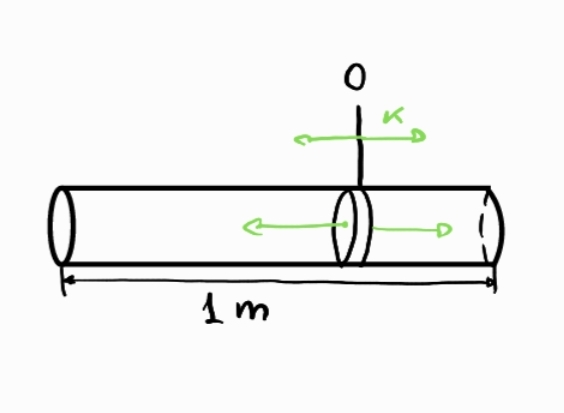
\includegraphics[scale=0.3]{EDP1.jpg}
\end{center}
$$ \cancel{P} = (P-\Delta P)(1+x)= \cancel{P} - \Delta P +xP -\underbrace{\Delta P}_{\sim 0} $$
$$ \Delta P = -xP $$
%creo que acaba de decir que va a hacer apuntes decentes
% Yo si fuera tú sudaría. idk por si acaso, si no comentamos todo

\end{document}
